% placeholder, will be updated soon

\section{STM32 based MCUs used in the project}
\label{sec:stm32_models_reasoning}
The first model of the STM32 used in the project, was the \href{https://www.st.com/en/microcontrollers-microprocessors/stm32f446.html}{STM32F446}, in combination with the \href{https://www.st.com/en/evaluation-tools/x-nucleo-cca02m2.html}{CCA02M2} extantion board.\\ The MCU was programmed to accquire the data signal from the microphones through the SAI peripheral, where the microphones were pairwaise connected to the same line, sending the data either at the rising edge of the common clock signal, or the falling edge. As presented in the section covering the SAI aquisition test, the signal sent by the MCU to the python based receiver, was contested to such a degree, that the DOA estimation wasn't able to reliably estimate the DOA of the strongest sound source. The group has also tried to implement the SPI in combination with I2C, to acquire the sound before the change in the MCU, which unfortunetly did not result in the correct sound acquisition. \\ % maybe add some more about that

This has led to change in the MCU to a \href{https://www.st.com/en/microcontrollers-microprocessors/stm32h743-753.html}{STM32H753} platform, which has a dedicated mode in the SAI peripheral for acquisition of the interleaved PDM signal from up to 6 microphones using the same SAI block. After many changes to the SAI, DMA configurations, and the main program for the MCU, the change in the signal sent to the receiver was non. The signal was still very highly correlated between the microphones on the same line, and the DOA estimation was random. The student has tried to use the \href{https://www.st.com/resource/en/user_manual/um2372-stm32cube-pdm2pcm-software-library-for-the-stm32f4f7h7-series-stmicroelectronics.pdf}{PDM2PCM} library, both by de-interleaving the signal before the PDM values were converted to the PCM format, and right after the conversion aswell. The resulting signal aqcuired by the receiver, was still unusable from the DOA estimation perspective, which has led to the chagne of the peripheral from SAI to DFSDM.\\

Originally the STM32H753 was meant to be used for implementation of the DFSDM, since it has a dedicated DFSDM module, but during the testing process of the MCU, the connectors for the USB were damaged, which has forced the student to change the MCU, to still be able to send the desired data load from the MCU to the receiver script.\\

The last MCU tested for audio acquisition in the project, and also applied in the final project design is the \href{https://www.st.com/en/microcontrollers-microprocessors/stm32f413-423.html}{STM32F413}. This MCU has two dedicated DFSDM modules, which also allow for higher number of microphones impemented in the system . This could be beneficiary if the system would be used to estimate the DOA in the three dimentional space. 
The MCU was also connected to the CCA02M2 extantion board, just as the two previous MCUs, to simplifie the signal acquisition from the micropohones. The main difference howerver, was that each microphone data pin was directly connected to its channel input at the MCU. In this way, the PDM values did not have to be manually de-interleaved before the PDM to PCM conversion. Since the MCU was to convert the PDM values into the PCM values inside of the DFSDM peripheral, there was no further need of applying the PDM2PCM library in the main code, which has simplified the debugging process. The MCU was the only one to correctly acquire the microphone signal, and managed to send it to the receiver so that the DOA could be correctly carried out. This has conviced the group to implement this MCU in the final design. 


% mention that the usb pins were damaged during the soldering process to defend the change to the f413
\section{Troubleshooting of the sound acquisition process based on the SAI}
\label{sec:troubleshooting_sound_acquisition}

The troubleshooting that ultimatley led to the change of the peripheral, was conducted due to the data signal from the microphones producing seamingly random DOA estimat of the strongest sound source. The system for audio acquisition, was then based on the STM32H753, which was connected to the CCA02M2 extantion board responsible for supplying, and handling the data from the microphones. The MCU SAI peripheral was generating the common clock signal for the microphones in the frequency of around 2 Mhz. The data pins from the microphones were connected pairwise on the data line, so that one microphone would send the data when the common clock signal was on the rising edge, and the other one, when the clock signal was on the falling edge. To achieve that, one of the microphones L/R pin had to be connected to the GND, while the other had to be connected to the 3.3V. \\

The first in the system to be controlled, was the above-mentioned L/R pin voltage levels. If both of the microphones in the pair would have the same voltage level on these pins, the data signal might be sent at the same moment, mixing the signals.\\
\newpage
The next to be controlled, was the code responsible for initialization of the filter handlers and their configuration. The code itself has changed several times during the troubleshooting proces, but one of the first initialization methods applied, can be accesed in Code~\ref{lst:filter_handler_config}.  

\begin{lstlisting}[style=cstyle, caption={Initialization of the filter handlers and their config}, label={lst:filter_handler_config}]
for (uint32_t index = 0; index < 2; index++)
	    {
	        PDM_FilterHandler[index].bit_order = PDM_FILTER_BIT_ORDER_MSB;
	        PDM_FilterHandler[index].endianness = PDM_FILTER_ENDIANNESS_BE;
	        PDM_FilterHandler[index].high_pass_tap = 1073741824; //2104533974
	        PDM_FilterHandler[index].in_ptr_channels = 2;
	        PDM_FilterHandler[index].out_ptr_channels = 2;

	        PDM_Filter_Init(&PDM_FilterHandler[index]);

	        PDM_FilterConfig[index].output_samples_number = 16;
	        PDM_FilterConfig[index].mic_gain = 0;
	        PDM_FilterConfig[index].decimation_factor = PDM_FILTER_DEC_FACTOR_64;

	        PDM_Filter_setConfig(&PDM_FilterHandler[index], &PDM_FilterConfig[index]);
	    }
\end{lstlisting}

The filter handlers were first planned to use a buffer per data line, that holds the interleaved values in the 8-bit format per microphone value, where the data from one microphone was to be indexed at the odd number, and the next one at the even number. Hence the \textbf{in\_ptr\_channels} and \textbf{out\_ptr\_channels} were both set to two, so that the handler would then return the PCM values using the same indexing logic, as for the input. During the testing however, it turned out that the values are very highly correlated, sugesting that the deinterleave of the values was not correct or simply lacking, which was later proven by lack of the above-mentioned function in the library, as seen in Figure~\ref{fig:fuckpdm2pcm}. 
 

\begin{figure}[h]
    \centering
    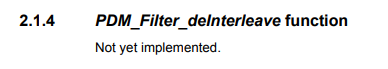
\includegraphics[width=0.5\linewidth]{Figures/pdm2pcmFUCKYOU.png}
    \caption{Lack of implementation of the deinterleave function in the PDM2PCM library. Source:\cite{st_um2372_pdm2pcm}}
    \label{fig:fuckpdm2pcm}
\end{figure}

The lack of dedicated deinterleave function, has forced the student to use selfmade function, which has also changed during the testing process, but one of the implementations can be seen in Code~\ref{lst:pdm_deinterleave_2_mics}.

\begin{lstlisting}[style=cstyle, caption={Method used to deinterleave two mics from one buffer at a time}, label={lst:pdm_deinterleave_2_mics}]
void PDM_Deinterleave_2_mics(const uint8_t *src, uint8_t *mic1, uint8_t *mic2,uint16_t len)
		{
			for (uint16_t i = 0; i < len; i += 2)
			{
				mic1[i/2] = ((uint8_t*)src)[i];
				mic2[i/2] = ((uint8_t*)src)[i + 1];
			}
		}
\end{lstlisting}
\newpage
After applying the above-mentioned method, the in\_ptr\_channel and out\_ptr\_channel were set to be equal one, as the buffers sent to the \textbf{PDM\_Filter} method were only expected to hold the data from one microphone, as seen in Code~\ref{lst:application_pdm_filter}.

\begin{lstlisting}[style=cstyle, caption={Application of the PDM\_Filter method}, label={lst:application_pdm_filter}]
 PDM_Filter(pdm_mic1, pcm_mic1, &PDM1_filter_handler);
 PDM_Filter(pdm_mic2, pcm_mic2, &PDM2_filter_handler);
 PDM_Filter(pdm_mic3, pcm_mic3, &PDM3_filter_handler);
 PDM_Filter(pdm_mic4, pcm_mic4, &PDM4_filter_handler);
\end{lstlisting}

Despite the application of several of deinterleave functions, and other changes to the code, the values sent by the MCU were still unable to produce a meaningfull DOA estimation. The correlation matrix from the results section, suggests that there was higher then expected correlation between the data signals on the same data line, which seams to caused by the incorrect channel separation or data leakage between the microphones. The easiest way to solve the issue at that time, seamed to be the change of the peripheral used by the MCU, which resulted in correct data signal acquistion and later quite precise DOA estimation.   
%
\section{Number of microphones used in the system}
From the begining of the design process, it was planned to use four microphones to accquire the acoustic signal around the tower, to later estimate the DOA of the incoming drone in a two dimentional space. The results prove that it is possible, and the estimated DOA is also quite accurate. It was however considered to expand the number of microphones used in the system, to increase the accuracy of DOA estimation and possibly add some redundency in the system, in case of failure of several microphones. It was also considered to use several independent units equiped with microphone arrays covering 360$\circ$ around each unit, which would be in constant communication with each other and the main tower. In this way the system would also be capable of estimating the distance of the drone and the main tower, by comparing the distances between units and their TDOAs. It is just a theroetical assumption that would have to be furtherly tested and reaserched on.      

\section{Change from UART to USB CDC}
In the early stages of the project, the UART was used to send the PCM data from the MCU to the receiver script. However during testing of the sound acquisition module, it was found that the payload per second, that the UART is capable of transmitting, is too low for then used desired sampling frequency. With four microphones, a 16-bit PCM samples with addition of a start and a stop bit per byte, and a desired sampling frequency of approx. 20 kHz, the recquired data payload would be as seen in Equation~\ref{eq:payload_no_overhead}.  

\begin{equation}
\label{eq:payload_no_overhead}
    payload = 20kHz \cdot 4 \cdot 2 \cdot 10 = 1.6Mbit/s
\end{equation}
\newpage
To acquire the desired 1.6Mbit/s of data, the baudrate of atleast 1.6 MBaud would be necessary. 
Accoridng to \cite{analog_uart}, the highest baudrate found in their table is 1.5 MBaud,  which would not satisfy the desired data transmition per second. It was assumed that maybe a higher baudrate could be applied, by the student was afraid that the data transmittion would be unstable, resulting in the loss of data. 
The later applied USB CDC FS, was able to transmitt the data in the speed of 12 Mbit/s as described in the theory section covering the USB, and as seen in Figure~\ref{fig:usb_fs}, which was the main why the USB CDC FS was applied in the final project.  

\begin{figure}[h]
    \centering
    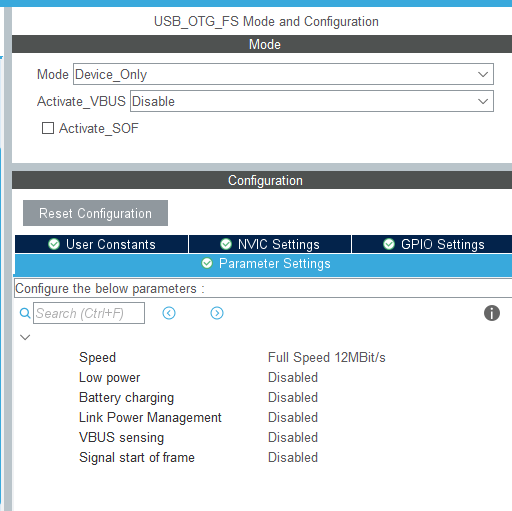
\includegraphics[width=0.5\linewidth]{Figures/speed_usb.png}
    \caption{Speed of the USB FS}
    \label{fig:usb_fs}
\end{figure}


%\section{sound pressure level measurements should have been conducted}

\section{Duration of the sound recording, and additional overhead in the system}
Duration of the sound recording varied, depending on which part of the system was tested and at which stage the test was conducted. During the early stages of the sound acquiering testig, when it was necessary to verify if the system is at all able to estiamte the DOA, the duration of 4 seconds per recording was used. In the later stages, when the DOA was proven to produce an accurate estimate, the duration has varied from 0.5s to around 1s per recording. At that stage the recordings of 0.5s durations were not reliable enough for the DOA to produce a correct estimate, so the group has sticked to the 1s durations for other tests aswell. After some consideration, the main reason for the unrealiable DOA estiamation using the 0.5s recording, seams to be the type of sound tested, which was the human speach and clapping sounds. This made it possible for the system to not catch the produced sound during the recording period.\\
\newpage
During the final test, when the recording period was set to 1s, the system has expirienced a significant lag between each DOA estimation, of around 3.4s per iteration. After the figure generating modules were deactivated in the system, the lag between each iteration was approx 1.26s, which proves that the main reason for the lag in the system was the generation and saving of DOA estimates, and Mel-spectrogram for each recording. This also proves that the easiest way to produce the DOA visualization, is simply by sending new estimated azimuth to the already initialized GUI.\\

\section{Wires used for the current design}
During the testing process the design used the following type of wires: \href{https://no.rs-online.com/web/p/breadboard-jumper-wires/7916454?cm_mmc=NO-PLA-DS3A-_-google-_-CSS_NO_EN_Pmax_Test-_--_-7916454&matchtype=&&gclsrc=aw.ds&gad_source=1&gad_campaignid=20298225819&gbraid=0AAAAADkeWNNR65FpdoBu5Vw5TPO3sZJXO&gclid=CjwKCAjw8arQBhB9EiwAfIKdQmniRsQJ3BquaxlQT0Hdzn6rzL6tpD5bGd_lQR6NpS9tRgIWoZC9VxoCEAQQAvD_BwE}{wire jumpers}. The wires are far from being perfect for high frequency data transmittion, due to lack of any additional protection against the EMI. In the final product, the transmittion wires would be changed to the F/FTP cabels, which according to \cite{linkpp_stp_cable_2025} use the foil shield per wire pair, and an additional foil shielding for the whole cable, which seams to be enough for the enviroment the product would find it self in.\\

Alternatively the data could also be transfered by the fiber-optic cables, which by design are completly resistant to the EMI, as they instead of carying the electrical signal, they carry the "light signal". However the eventual use of the fiber-optic cable, would introduce additional complexity in the electronical desing in form of an aditional fiber optic converter, which increases the total cost per unit.     


\section{Redesign of the upper PCB}
The final version of the PCB as demonstrated in the method section, has eveloved from another version seen in Figure~\ref{fig:the_old_upper_pcb}. The previous design, was meant to include the \href{https://no.rs-online.com/web/p/power-motor-robotics-development-tools/1360748}{Stepper 2 Click} motor controller based on the \href{https://www.pololu.com/file/0j450/a4988_dmos_microstepping_driver_with_translator.pdf}{A4988} chip to control the stepper motors. 

\begin{figure}[h]
    \centering
    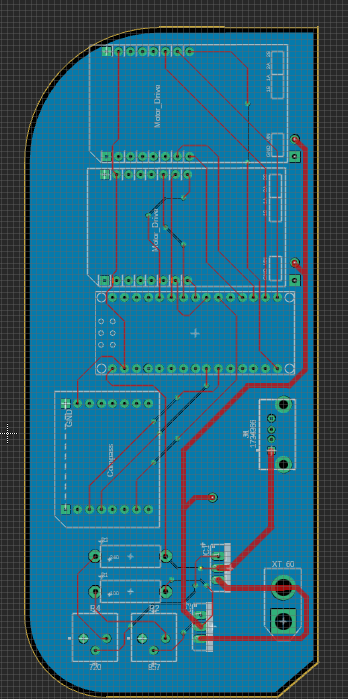
\includegraphics[width=0.25\linewidth, angle=-90]{Figures/old_upper_design.png}
    \caption[The old upper PCB design]{The old upper PCB design, using the A4988 based motor controller}
    \label{fig:the_old_upper_pcb}
\end{figure}
\newpage
The main reason for the change of the motor controller to the L6205N, was that during the PCB testing the controller has never managed to drive the stepper motor used in the design. The controller itself was rapidly heating up when being applied the signal voltage, which might suggest the internal overcurrent protection system was shuting down the control circuit. After the troubleshooting of the system, the easiest solution to that problem, seamed to be the application of the L6205N, which would be protected by the protection system applied in the LM338 voltage regulator. 

\section{Use of The bottom PCB as a substitute of the CCA02M2 extation board}
The CCA02M2 which was used in the early stages of the project, was meant to be replaced by the bottom PCB design shown in the method section. The reason for that was the reduction of the number of wires used in the system, as they were assumed to be more exposed to the EMI, then the PCB itself. The other reason was the design of the tower, which would only allow the CCA02M2 to be mounted on top of the STM32, if the walls of the bottom tower part were made even taller, to make sure that the gears from the upper part would not get in contact with the wires, or other sticking parts from the extantion board.


\section{Distance detection of the sound source}
The system currently does not allow for the distance detetion of the incoming drone solely based on the acoustic data. In the current design the distance to the drone may only be estimated based on the camera feed.

\section{Prediction of the future DOA based on the rate of change - NOT DONE}

.............

\section{Use of threads in the program}
The current program design for sound acquistion and processing, as seen in the flowcharts included in the methods section, is sequenctional. This forces the program to execute each consecutive step such as MFCC extraction and the DOA estimation, before the new sound could be recorded and processed. This creates the additional lag and inaccuracy in the DOA estimation, as the estimated DOA represents the position of the drone at start of the iteration, and not necessarily the drone position after the full processing pipeline has finished.\\

A threaded design could reduce this problem by allowing one thread to continously receive or buffer the new audio samples, while another thread would be processing already acquired sound signal. A possible application would be a producer-consumer structrue, where the audio receiver would act as the producer, which continously reads the incoming PCM samples from the STM32 MCU, and would place the complete audio frames into a shared queue. The part of the program responsible for the signal processong, would then act as the consumer, taking the oldest available audio frame from the queue, and would perform the necessary conversions and processing. In this way the new data could be acquired, while the processing modules would be processing the previously sampled data. As a result the created gaps between the readings could be reduced. Based on explenation from \cite{anderson_producer_consumer_python}. 

\section{Use of beta value for PHAT - NOT DONE}
The PHAT weighiting............

\section{frequency mask for PHAT weighting}
The frequency mask used in the PHAT weighting is currently excluding the signal values otside of the desired frequency band of between 80 to 6000 Hz. The upper limit chosen arbitrary during the testing stage, as the students lacked the reliable infromation on which frequency bands were present in the sound produced by drone available in the laboratory. The lower limit of 80 Hz, was applied to reduce the eventual influence of the power lines, which operate at the frequency level of 50 Hz. After the final test, it may be concluded that the band interval may be reduced from 6000 Hz, to less then 4000 Hz to furtherly reduce the influence of the noisy frequnecy bands. This may however have quite negative influence onto the detection system, if the drone to be detected would produce acoustic signal, where most of energy would be found in the high frequency bands.  









%For the end product, the bottom PCB seen in Figure~\ref{fig:3d_model_bottom_pcb} would be applied instead of the CCA02M2 board.
%\section{The reason for the applied distance between the microphones and the platforms center}
%\section{Use of the preemphesized signal for mfcc and the original signal for log-mel}
% i forgot to change the signal type, when i have added the preemphesis :P . 
%\section{Use of different mfcc coeffs}
%\section{Use of a 32-bit word as the DMA buffer}
%\section{The reason why The bottom PCB was not included in the final project}
%\section{Idea of using the rotory microphone system}
%\section{Reduction of the frequency mask interval for the phat weighting filter}
%, but based on the frequency bands present during the test, the band-pass could be safely reduced from 6000 Hz, to maybe even 1000 Hz.
% mics go around


\section{Raspberry PI and YOLO performance}

The hardware benchmarking results demonstrate that a Raspberry Pi 5 running YOLOv8n inference purely on the CPU is insufficient for real-time drone tracking, while the addition of the Hailo AI accelerator brings performance well within an acceptable operational range. (\ref{fig:Interference_comp}) At an average inference time of 235.6ms, the CPU-only pipeline achieves approximately 4.25 frames per second, which is too slow for smooth tracking, which would cause problems in cases of rapid drone movement. (\ref{fig:Interference_comp}) The Hailo-accelerated pipeline, by contrast, achieves an average inference time of 9.2ms, corresponding to approximately 108 frames per second, far exceeding the minimum threshold typically associated with real-time object tracking. (\ref{fig:Interference_comp})

 \vspace{1em}
 
CPU usage and temperature also carry implications for deployement. In the CPU-only configuration, the CPU usage averaged at 92.5\%, leaving little room for other system processes. (\ref{fig:cpu_usage_comparison}) By contrast, by using the HAILO chip to offload the interference, the CPU usage declined to 29.7\% giving the system more headroom for other processes and applications, as well as potential future expansions of the program. (\ref{fig:cpu_usage_comparison}) The CPU temperature results reinforce this picture: the CPU-only configuration showed a steadily rising temperature that stabilised around 73°C, a level that risks thermal throttling in enclosed or low-airflow enclosures typical of embedded systems.(\ref{fig:cpu_temp_comparison}) The Hailo configuration maintained a stable 54°C with no upward trend, suggesting reliable sustained operation. (\ref{fig:cpu_temp_comparison}) 

 \vspace{1em}
 
The RAM overhead introduced by the Hailo pipeline, approximately 140 MB higher on average than the CPU-only configuration, is the one metric that marginally favours the CPU-only approach. (\ref{fig:RAM Usage}) However, given the 8GB RAM available on the Raspberry Pi 5, this difference is negligible in practice and does not affect the overall conclusion. On the other hand, the RAM usage in both configurations utilised close to 4GB of RAM (\ref{fig:RAM Usage}), indicating that 8GB of RAM is the minimum amount of system RAM to be used for drone detection. 

\vspace{1em}

It should also be noted that the model quantization during the ONNX 
to HEF conversion was performed using randomly generated calibration 
data via the \texttt{--use-random-calib-set} flag, rather than a 
representative set of real drone images. Proper quantization 
calibration using images from the training dataset would allow the 
compiler to derive more accurate activation statistics, and would 
likely reduce the accuracy loss introduced by the 32-bit to 8-bit 
weight quantization, potentially improving detection confidence 
and bounding box precision during inference on the Hailo hardware.

 \vspace{1em}

 Taken together, these results suggest that for a low-cost real-time drone detection and tracking system, the minimum viable hardware configuration is a Raspberry Pi 5 paired with a Hailo AI accelerator. The CPU-only Raspberry Pi 5, despite being a capable single-board computer, cannot sustain the inference throughput required for reliable tracking. The Hailo chip is a relatively low-cost dedicated neural network accelerator, and its inclusion transforms an otherwise insufficient platform into one capable of smooth real-time inference with substantial CPU headroom remaining for system integration
 
  \vspace{1em}
  
The camera tracking system was not completed on time due to issues with controlling the stepper motor, with the most likely culprit being the voltage given on the 10V rail, which was measured to be at 12V. The exact reason for this is unclear, altough mostly likely it is due to a faulty component and not the design itself. This most likely caused the voltage regulator to overheat, as well as the stepper motors to jitter. However, The stepper motors still moved enough to confirm that the Pan and Tilt function worked as designed.

In most camera sensor solutions for drone detection, higher quality cameras with optical zoom are often optimized, as that would increase the range of the drone detection system. 



\section{Drone detection performance}

The results demonstrate that the YOLOv8n achieved a stronger performance on the drone detection dataset (\cite{DroneDatasetFinal}) in comparison to the MobileNet V1 model used in the original paper. The YOLOv8n model avhieved a mAP@50 of 0.832, compared to the 0.533 of the highest performing MobileNet V1 model (\cite{DroneDatasetFinal}). The peak F1 score (\ref{tab:yolo_detection_performance}) of 0.81 at a confidence threshold of 0.571 exceeds the original papers maximum of 0.602. Both models were trained and tested on the same datasets, with the difference being attributed to improvements within object detection model architecture.


MobileNet V1 was originally proposed by \cite{howard2017mobilenets} in 2017 as a lightweight architecture designed primarily for mobile and embedded applications (\cite{howard2017mobilenets}). The SSD detection framework it was paired with predates many advances which have now become standard in object detection models.YOLOv8, released by Ultralytics in 2023, incorporates a CSPDarknet-based backbone, a Feature Pyramid Network combined with a Path Aggregation Network in the neck for multi-scale feature fusion, and an anchor-free decoupled detection head that independently handles classification and bounding box regression — removing the need for predefined anchor templates and reducing post-processing overhead (\cite{terven2023comprehensive, jocher2023yolov8}). These advance,s as well as a more refined training pipeline, represent the progress made within the field of object detection. The results of the original papers performance in comparison to the one presented in this study is reflective of the generational gap within object detection algorithms.   

 \vspace{1em}

Another possible contribution to the improved results is the higher input resolution used in this study, 640x640, in comparison to the original papers 300x300 (\cite{DroneDatasetFinal}). Since the dataset contains a high proportion of images where the drone appears small, a higher resolution is advantagous since it preserves more of the spatial details. The augmentation strategy, including mosaic augmentation, scale jitter, and rotation, is well-suited to the dataset's variability in drone size, viewing angle, and background environment.

Selection of the dataset was found to be the most critical factor across the training process, as multiple models were trained on different datasets before arriving at the final configuration. The dataset used was selected because it produced the model with the fewest false positives, with the key advantage being the large number of background-only images in the validation set. These negatives actively penalise the model for spurious detections during training, encouraging greater specificity (\cite{DroneDatasetFinal}). This effect is also visible in the validation loss curves, where the classification loss showed an anomalously high scale (~16–27) compared to the training classification loss (~0.40), directly attributable to the 2,750 background-only images in the validation set penalising false detections (\ref{fig:pYolo_results}).

\vspace{1em}

The normalised confusion matrix shows that all background instances in the test set were assigned a non-zero detection at some confidence level, indicating some false positives(\ref{fig:Yolo_confusion_matrix}). At the recommended threshold of 0.571 this behaviour is well controlled, as the precision confidence curve shows high precision, low false positives, in this region. (\ref{fig:pr_curve}). 

The precision-recall curve illustrates that the model maintains near-perfect precision across a wide recall range before degrading sharply beyond approximately 0.75 recall, indicating confidence and accuracy on the majority of detections with uncertainty concentrated at harder examples. The F1-confidence curve shows a broad plateau between roughly 0.3 and 0.7 confidence, suggesting the model is not overly sensitive to the exact choice of threshold within this range, which is a practically useful property for deployment. The recall-confidence curve reveals a notable strength: at near-zero confidence threshold the model achieves a recall of 0.94, meaning it detects the vast majority of drones present in the images before any filtering is applied. For a security-oriented application such as drone detection, high recall is generally prioritised over precision, as missing a drone carries greater risk than generating a false alarm.

\vspace{1em}

The mAP@0.5 score of 0.832 indicates that the model detects drones reliably, but the mAP@0.5:0.95 score of 0.420 indicates that the predicted bounding boxes are not always tightly localised \ref{tab:yolo_detection_performance}. This difference can be attributed to the difficulty of creating precise boxes for small objects. This poses a potential challenge for drone tracking applications where an accurate position estimate is required. However, for the intended use case of keeping the drone within the camera frame, imprecise localisation may be less critical provided the detection itself is reliable. The paper does not report mAP@0.5:0.95, so a direct comparison at this stricter threshold is not possible, though it is reported here for completeness. Another solution to this could be the investment in a high quality camera with a high optical zoom, altough that would most likely increase the cost of the system significantly. 

\vspace{1em}

The false positives seen in Real-world inference testing further highlighted the dataset's influence on model behaviour. The false positives observed in the Floureon FPV video \cite{floureon2017} can most likely be attributed to the dataset lacking sufficient images of drones against darker tree backgrounds \cite{DroneDatasetFinal} (\ref{fig:video_comparison}). Similarly, in the TED talk video \cite{dandrea2016}, which features a darker indoor environment cluttered with people, the elevated false positive rate likely reflects the absence of indoor drone footage in the training data. These failure cases highlight the necessity of datasets that cover a diverse range of backgrounds and lighting conditions, and suggest that targeted data augmentation or dataset expansion in these specific scenarios could improve robustness. 

\vspace{1em}

The limited scope of the live detection test reflects the state of 
the system at the time of testing rather than a fundamental limitation 
of the approach. A more rigorous evaluation of the visual detection 
subsystem would require a different experimental setup. Future testing 
should be conducted outdoors in environments representative of the 
system's intended use case --- private property, suburban areas, 
open fields, and urban settings where unauthorised drone activity 
poses the most common threat to individuals and small organisations. 
These environments also provide the backgrounds most relevant to 
the training dataset (\cite{DroneDatasetFinal}), including open sky, 
buildings, trees, and varied terrain, which should improve detection 
reliability compared to the cluttered indoor laboratory setting 
used here. The test drone should be a standard consumer quadcopter 
of the type well-represented in the dataset, rather than the 
irregular laboratory drone used in the initial test. The standard consumer quadcopters fits more with the intended use case, as these are the drones that are more of a threat towards civilians. Detection 
performance should be evaluated at several measured distances, 
for example at 10~m, 25~m, 50~m, and 100~m intervals, to 
characterise how detection confidence and bounding box precision 
degrade with range. This would also allow a meaningful assessment 
of whether the mAP@0.50:0.95 score of 0.420 --- which indicates 
imprecise bounding box localisation on small targets --- represents 
a practical limitation for the tracking application, where only 
the centre pixel coordinate is required rather than a tight 
bounding box. Finally, a complete end-to-end test with the motor 
tracking operational would allow evaluation of the full 
coarse-to-fine pipeline: acoustic DOA orienting the camera, 
followed by YOLO-driven continuous tracking, with the latency 
and angular accuracy of each stage measured independently.

\vspace{1em}

Finally, training time was a practical bottleneck throughout this project, limiting the number of training runs and the degree to which hyperparameters could be systematically explored. The NVIDIA RTX 4050 laptop GPU, while sufficient to complete training, imposed meaningful constraints on iteration speed. It is recommended that future work utilise a more powerful GPU, as this would significantly reduce training time and allow more thorough hyperparameter search and experimentation.

\section{Hardware cost comparison}

A notable gap in the existing literature on vision-based drone detection is the limited reporting of hardware costs alongside detection performance metrics. Most academic work focuses on algorithm design and benchmark accuracy, with few studies providing an itemised hardware cost for their proposed systems. One exception is the RF-based system by (\cite{swinney2022lowcost}), which explicitly reports a total edge node cost of under €490 (~kr. 5,290), though at the cost of inference times of 15–28 seconds that preclude real-time tracking (\cite{swinney2022lowcost}). Commercial drone detection solutions offer substantially higher performance but at prices that are orders of magnitude greater, with EO/IR camera systems ranging from approximately €9,000 to €72,000 (~kr. 97,000–778,000) and radar-based systems from €27,000 to over €450,000 (~kr. 292,000–4,860,000) \cite{airsight2025buyersguide}.

The system proposed in this work achieves real-time drone 
detection through the combination of acoustic direction of 
arrival estimation using a four-element MEMS microphone 
array and visual detection at approximately 108 frames per 
second using the Hailo AI HAT+ accelerator 
(\ref{fig:Interference_comp}), at a total system hardware cost of 
approximately €830 (~NOK~8,503). This represents a substantial 
reduction in cost relative to both commercial alternatives 
and the performance threshold required for practical tracking 
applications, while simultaneously providing the 
complementary strengths of omnidirectional acoustic coverage 
independent of lighting conditions and real-time visual 
confirmation with precise pixel-level localisation 
(\cite{seidaliyeva2024advances, macedo2025drone}).
\vspace{1em}


The lack of hardware cost reporting in the audio-visual drone detection literature is a recurring limitation. Svanström et al. (2020), one of the most cited multi-sensor drone detection studies combining visible, thermal, and acoustic sensors, provides no hardware cost breakdown \cite{svanstrom2020realtime}. Similarly, Ding et al. (2023) describe their acoustic-optical fusion system MUTES as having "acceptable cost" without providing specific figures \cite{ding2023drone}. This makes direct cost comparison with the system proposed in this work difficult. The absence of cost reporting in academic literature likely reflects a research culture that prioritises algorithmic performance over deployment economics, despite the practical importance of cost for the widespread adoption of drone detection systems at critical infrastructure.


\section{Sensor fusion synergy}

The combination of acoustic and visual sensing employed in this project follows 
the principle of multimodal drone detection, where each sensor modality compensates 
for the limitations of the other (\cite{seidaliyeva2024advances}). This approach 
is supported by the work of Ding et al., who proposed the MUTES system combining 
a microphone array, camera, and lidar for drone detection and tracking, employing 
a coarse-to-fine localization strategy in which acoustic direction estimation 
activates and steers the optical modules toward the target 
(\cite{ding2023drone}). Their results demonstrated that sensor fusion achieves 
higher accuracy than any individual modality alone, with a 3D positioning error 
of less than 1.5\% of the detection range (\cite{ding2023drone}).

The combination of acoustic DOA estimation and visual YOLO detection in this 
project provides complementary strengths that neither sensor achieves 
independently (\cite{seidaliyeva2024advances, macedo2025drone}). The microphone 
array can detect a drone beyond the camera's field of view and provide a 
directional estimate before the drone is visible, allowing the camera platform 
to orient towards the target (\cite{ding2023drone}). The camera then provides 
visual confirmation and precise pixel-level localisation, which reduces false 
positives from the acoustic classifier (\cite{seidaliyeva2024advances}). The 
acoustic subsystem provides omnidirectional coverage independent of lighting 
conditions and without requiring line of sight (\cite{ding2023drone}), while 
the camera subsystem provides visual confirmation and precise localisation 
(\cite{seidaliyeva2024advances, macedo2025drone}).

This sensor fusion approach is particularly valuable in low-cost systems where 
neither sensor alone is sufficiently reliable (\cite{macedo2025drone}). The 
acoustic system struggles with background noise 
(\cite{macedo2025drone, seidaliyeva2024advances}), while the camera struggles 
with small, fast-moving targets at distance and produces false positives in 
cluttered environments (\cite{macedo2025drone}). Their combination addresses 
the primary failure modes of each modality 
(\cite{seidaliyeva2024advances, macedo2025drone}), and multimodal approaches 
of this kind have been shown to achieve positioning errors below 1.5\% of 
detection range (\cite{ding2023drone}), representing a significant improvement 
over single-modality systems.

\section{GUI}
The GUI was originally intended to run on a Raspberry-Pi. During the final weeks of development the device began to overheat and started smooking, prompting us to discontinue its use because it risked further damage and could delay the project further. This also meant that the initial plan to build with the possibility to interconnect several Raspberry-Pis as a microphone‑array field could not be realised.
The server was containerised with Docker to simplify updates and to maintain compatibility with a Raspberry-Pi. Since the Raspberry-Pi was ultimately not employed, the Docker‑based implementation contributed little to the final system.

\vspace{1em}

The GUI also incorporated an SSH certificate to allow GPS coordinates to be transmitted without modifying the user’s browser. However, the absence of an Internet router that could be configured for port‑forwarding prevented us from exposing the web server beyond a localhost address.

\vspace{1em}

Although the GUI includes a fully functional Open‑Stream‑Map integration for visualising drones, the current implementation cannot reliably estimate distances; consequently, it cannot place accurate markers on the map. A possible remedy would be to represent positional uncertainty, for example by displaying a line that indicates the potential trajectory of a drone, or by rendering a cone that shows angular uncertainty (see Figure 5.17.1).


\begin{figure}[H]
    \centering
    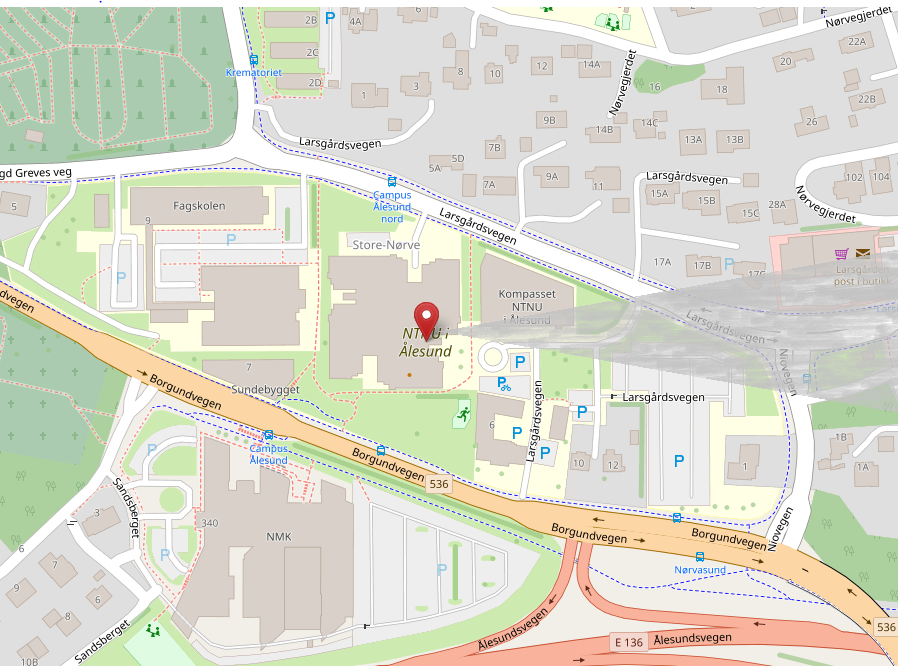
\includegraphics[width=0.5\linewidth]{Figures/Brage/mappEksempelSearchCone.png}
    \caption{Example for how a search cone showing angular uncertainty on the map could look, where the gray cone is the possible location of found drone}
    \label{fig:placeholder}
\end{figure}

Because the SSH certificate could not be deployed, the webserver does not have ample security measures. This lacking implementation represents a further development target, where the implementation of certification and stricter access-control policies should be prioritized. Nevertheless, the limited security exposure the system experiences given it is run locally means the lacking security measures does not affect the validity of the experimental results.

\section{Temp name}
As originally planned, the system was to run on two Raspberry-Pis: one dedicated to the camera and a second responsible for the web server, machine‑learning‑based sound classification, and connection to the microphone array. During integration the Raspberry-Pi designated for the primary subsystem overheated, so we migrated the live‑system test to a laptop.

This migration introduced a new problem: the newer TensorFlow release is not compatible with Windows, which forced operation in an environment with an older Python interpreter (version 3.10.20). Consequently, several dependent libraries also had to be downgraded.


The Python environment was managed with Conda to keep the package versions reproducible. Because of the version changes, The CNN loading procedure needed a minor modification: rather than loading a saved model object directly, the model architecture was initialized then was supplied the trained weight.Despite these adjustments, no functional shortcomings were observed; the system performed as expected in all preceding tests. Since the laptop exhibited no accuracy degradation and the Conda environment differs only marginally from the Raspberry-Pi setup, there is no substantial obstacle to eventually deploying the complete system on a single Raspberry-Pi. 
 
